\documentclass[12pt,letterpaper]{article}
\usepackage{titling}
\usepackage{amsmath}
\usepackage{amssymb} 
\usepackage{graphicx} % For image
\usepackage{float} % For image H option
\usepackage{enumitem} % For enumerate
\usepackage{bm} % For bold math symbols
\usepackage{xcolor} % For color
\usepackage[margin=1in]{geometry}


\begin{document}
\title{\textbf{Segmentation of Vessels in Retinal Images}}
\author{Team Members: Shiyu Wang, Enhao He, Jiacheng Ma, Joe Wang}
\date{}
\setlength{\droptitle}{-2.75cm}
\maketitle
\vspace{-2cm}


\section{Methods}
\subsection{K-means Clustering}
\subsubsection{Find the Best ``n\_clusters''}
Try to decide the best numbers of clusters by comparing the mean of the AUC value of the 20 figures. 
\begin{center}
    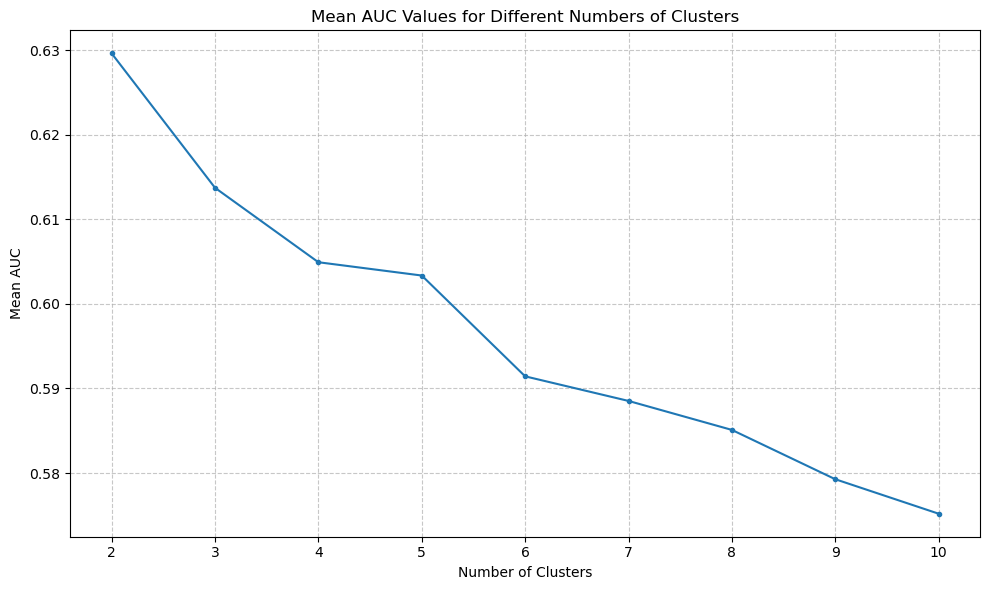
\includegraphics[scale=0.6]{Figures/1-1 Find the Best n_clusters.png}
\end{center}
The line is descending. At least 2. But 2 doesn't perform well. 
\begin{center}
    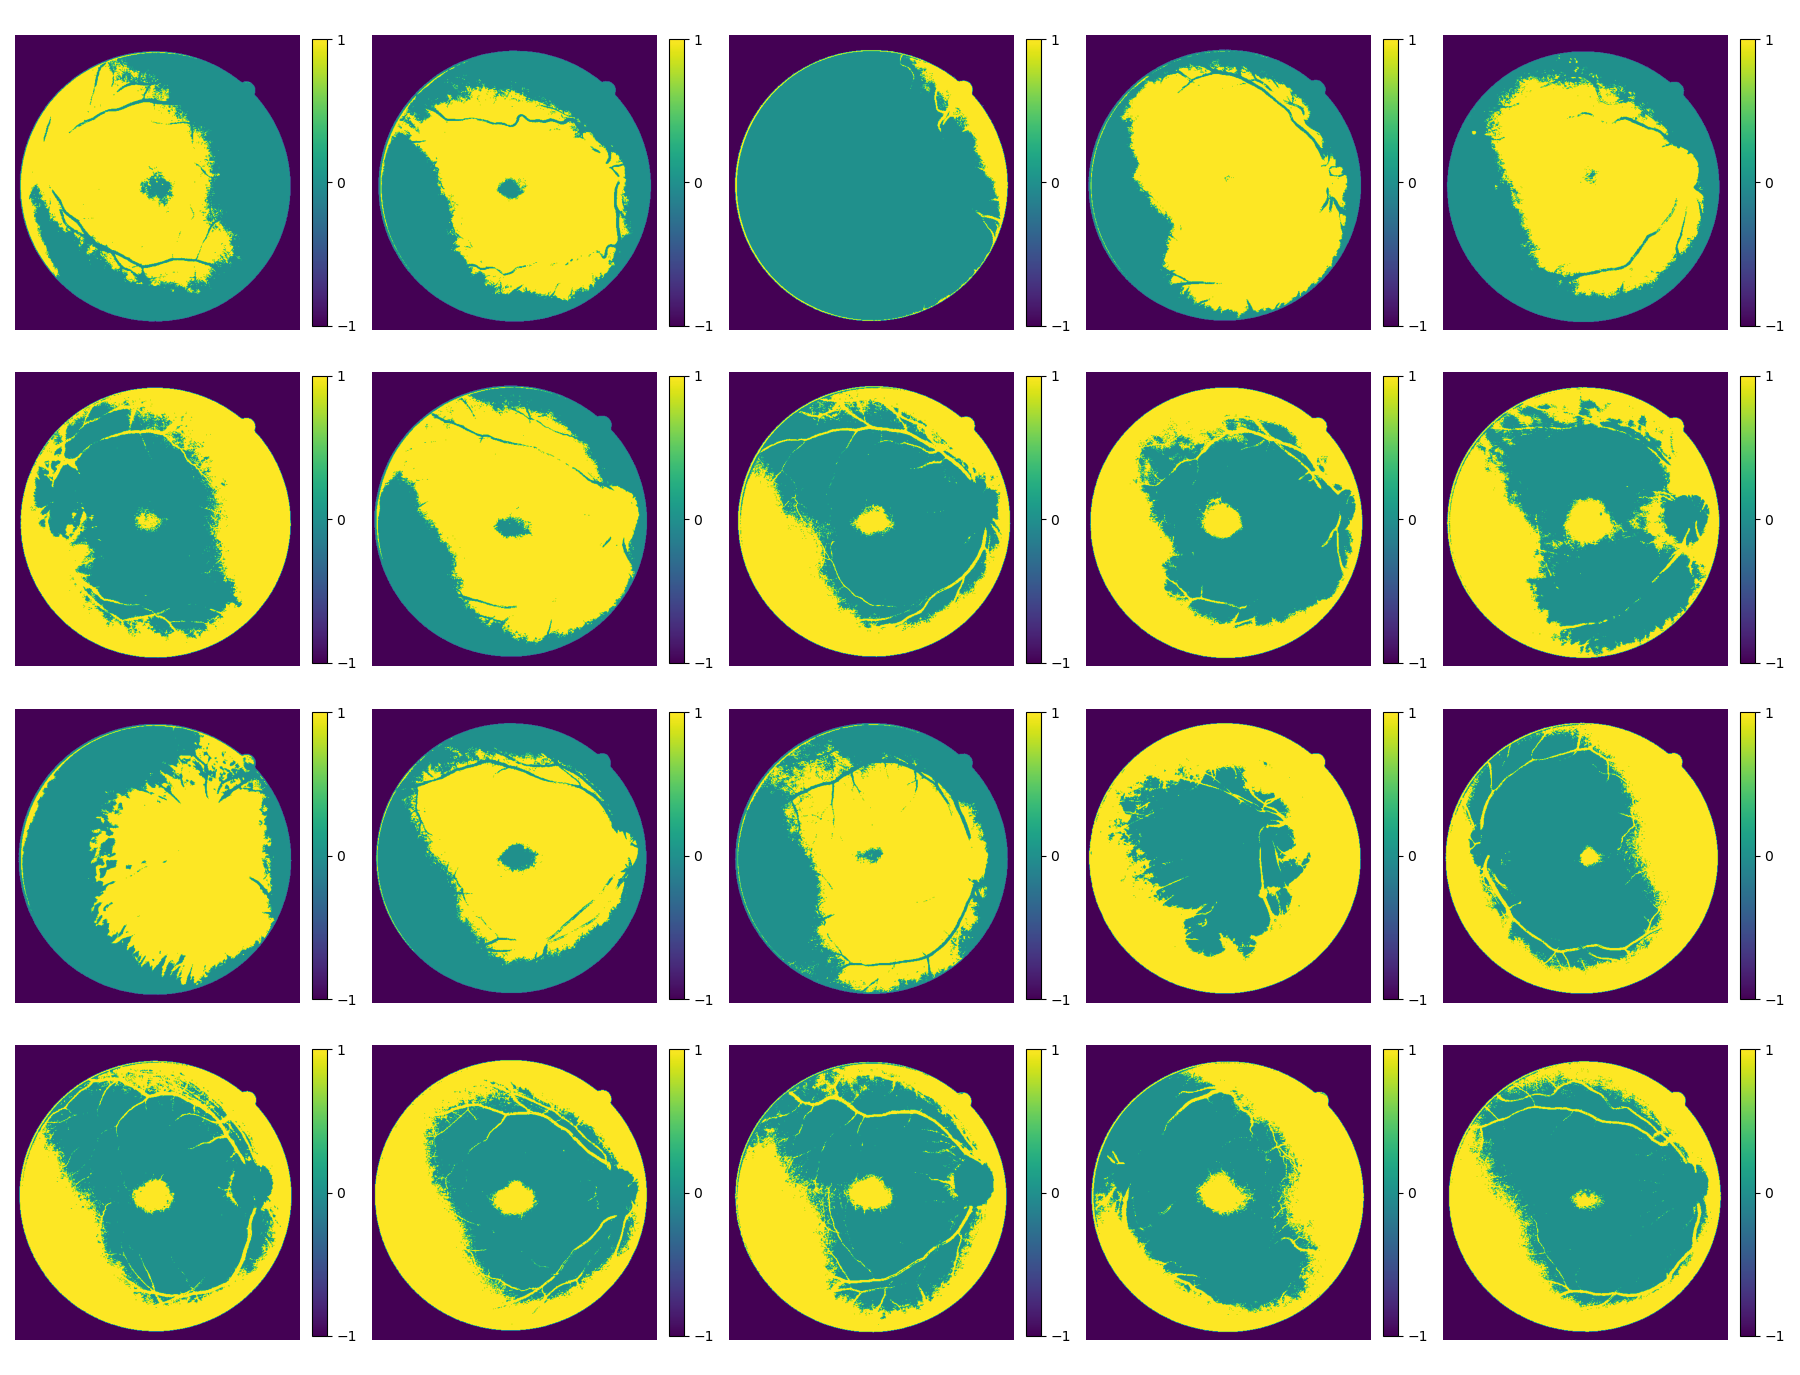
\includegraphics[scale=0.3]{Figures/1-2 2 Clusters.png}
\end{center}
Then we increase the n\_clusters. 
\begin{center}
    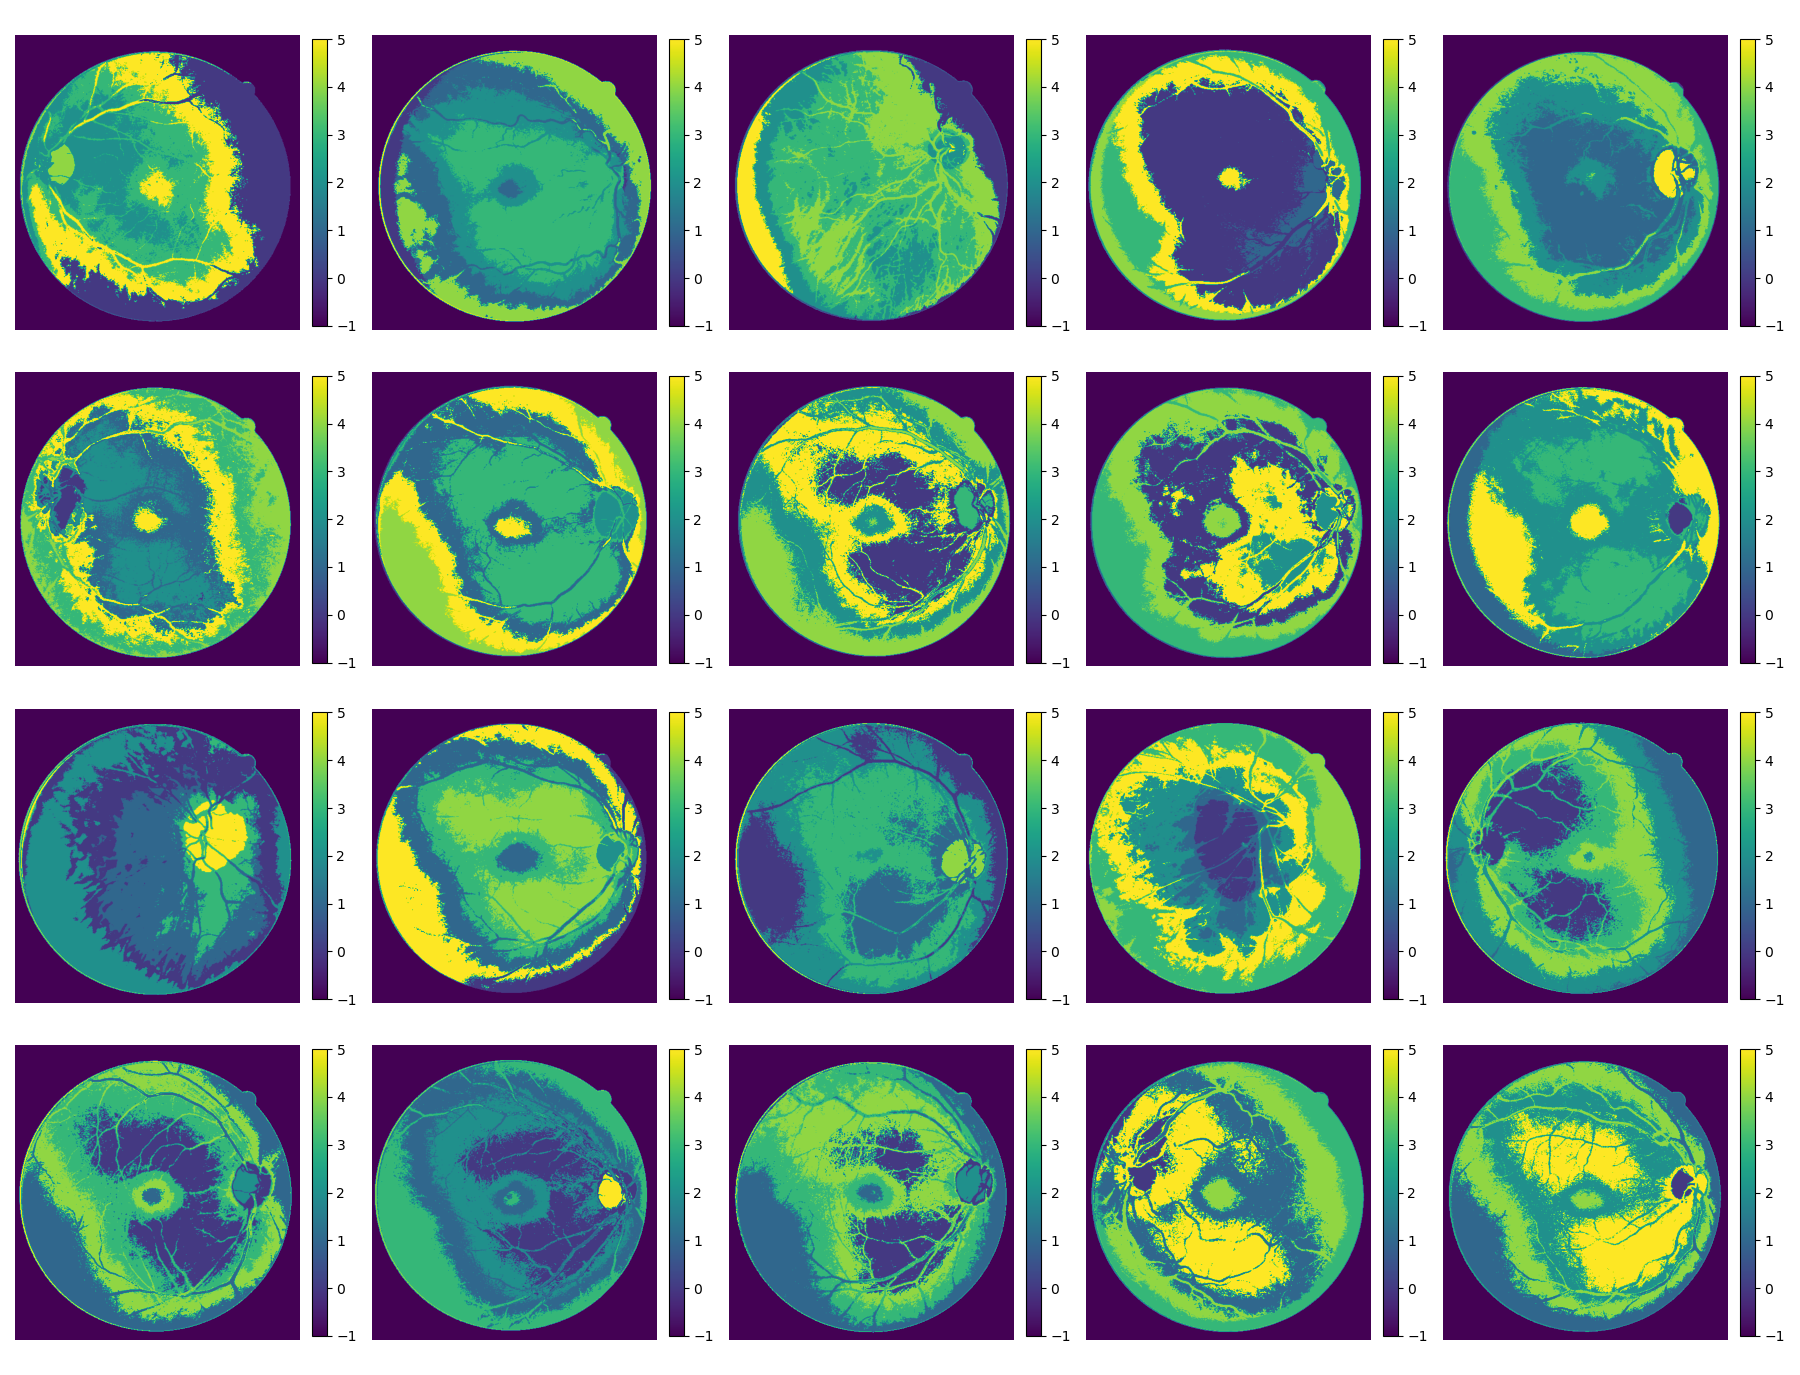
\includegraphics[scale=0.3]{Figures/1-2 6 Clusters.png}
    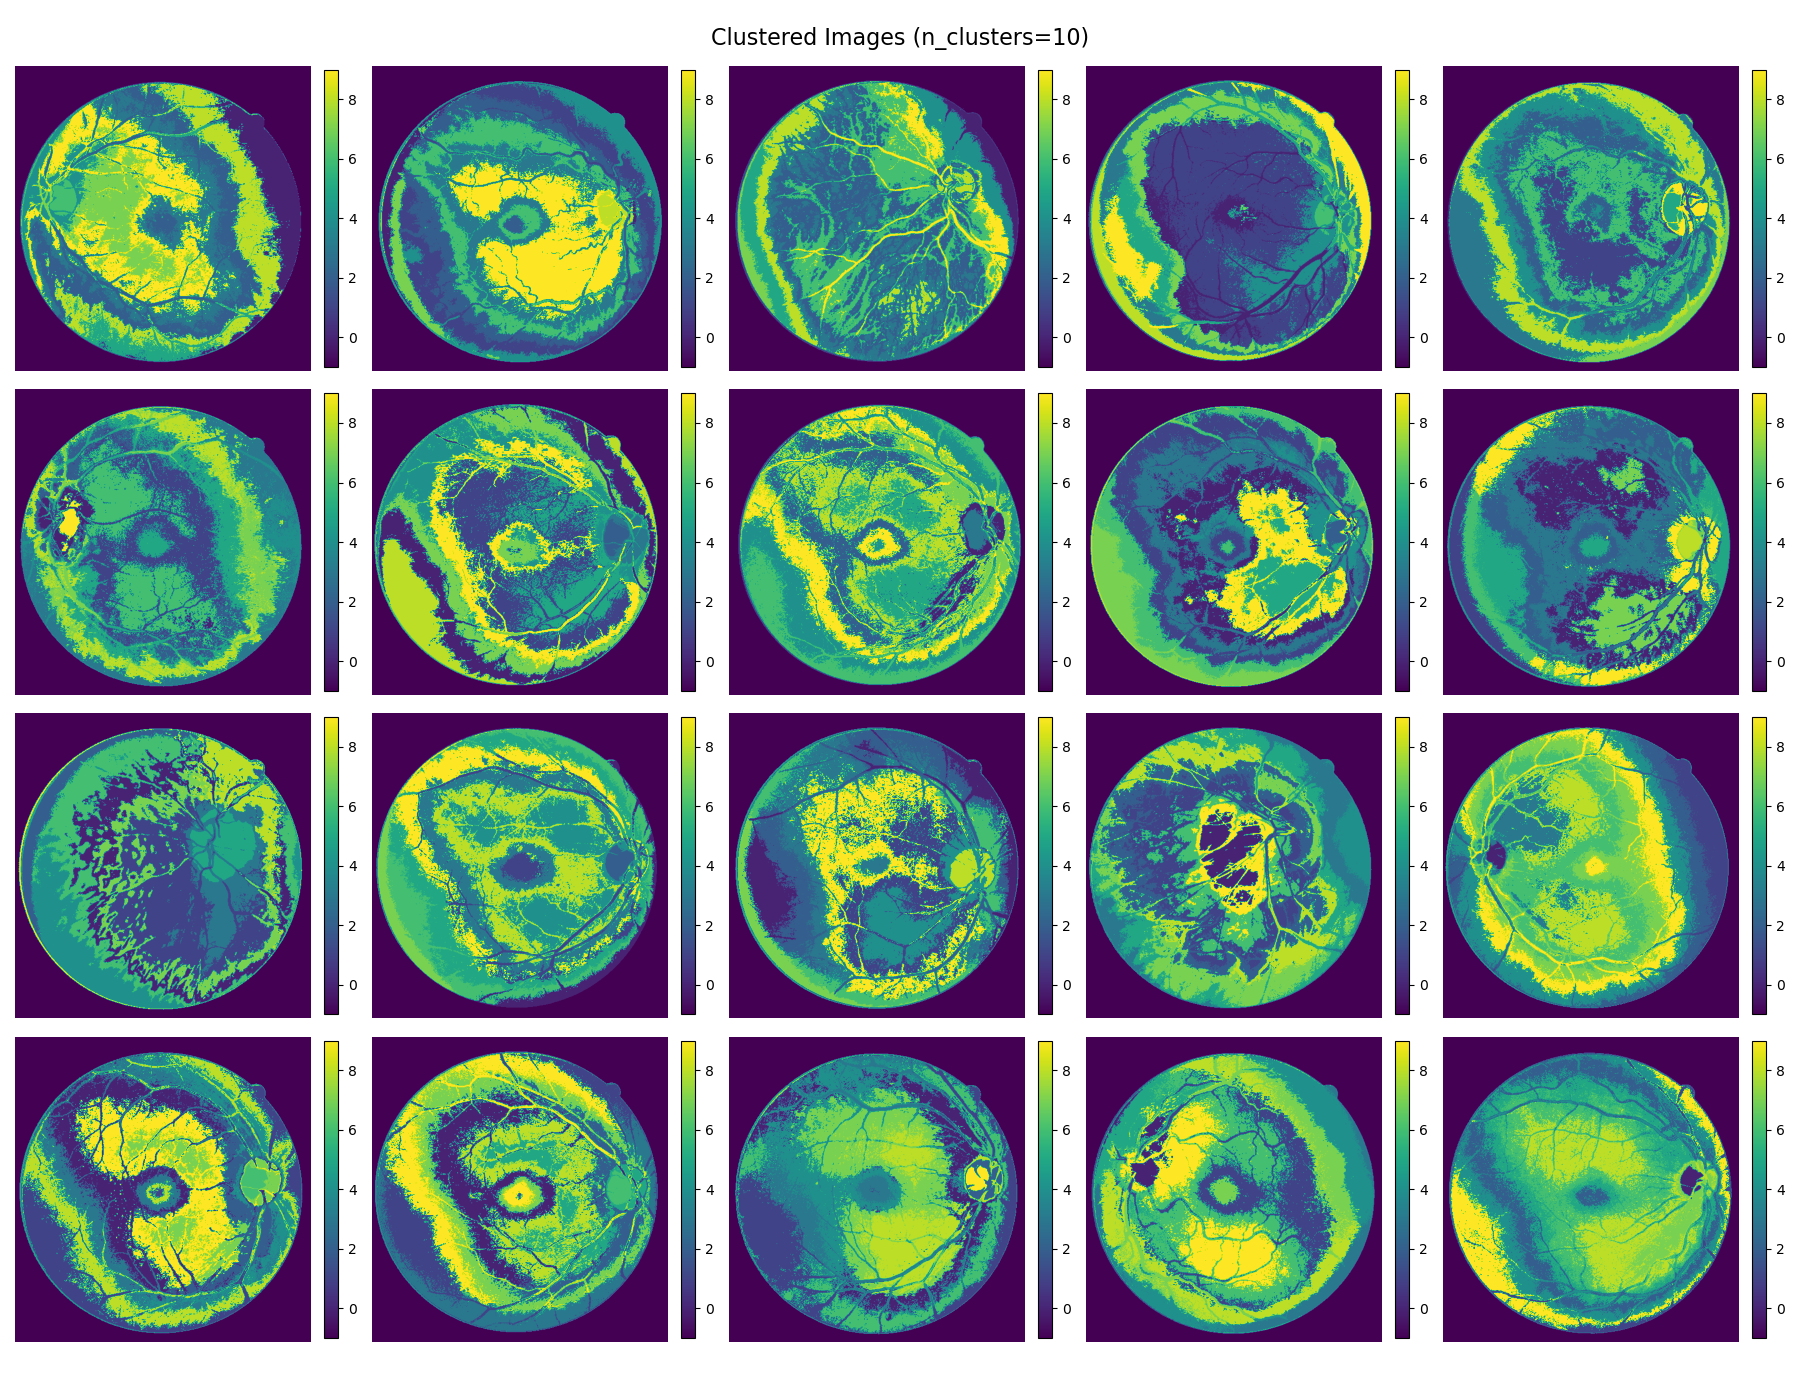
\includegraphics[scale=0.3]{Figures/1-2 10 Clusters.png}
\end{center}
We finally choose 10 because of its performance, but there still are some problems: the vessels' pixel are contained in many different clusters. \\
Here is a special case: 
\begin{center}
    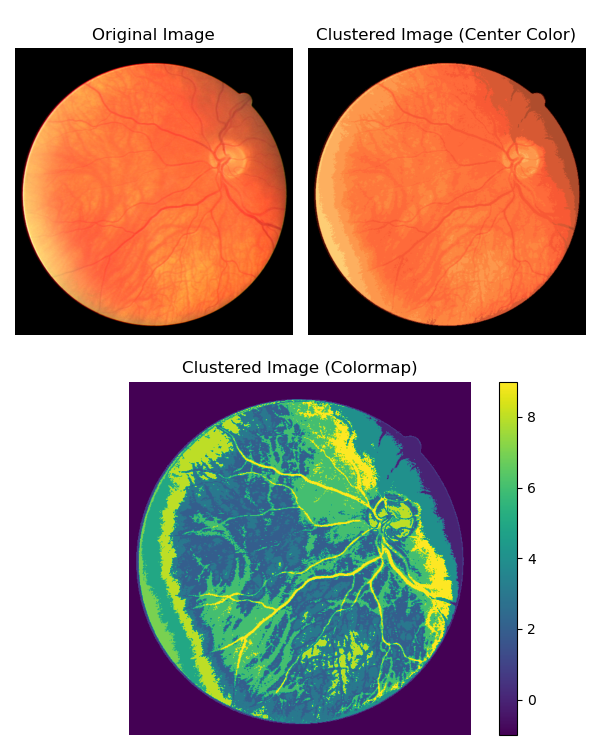
\includegraphics[scale=0.5]{Figures/2 10 Clusters.png}
\end{center}


\subsubsection{Use the Optimized K-means Algorithm}
The best three examples are:
\begin{center}
    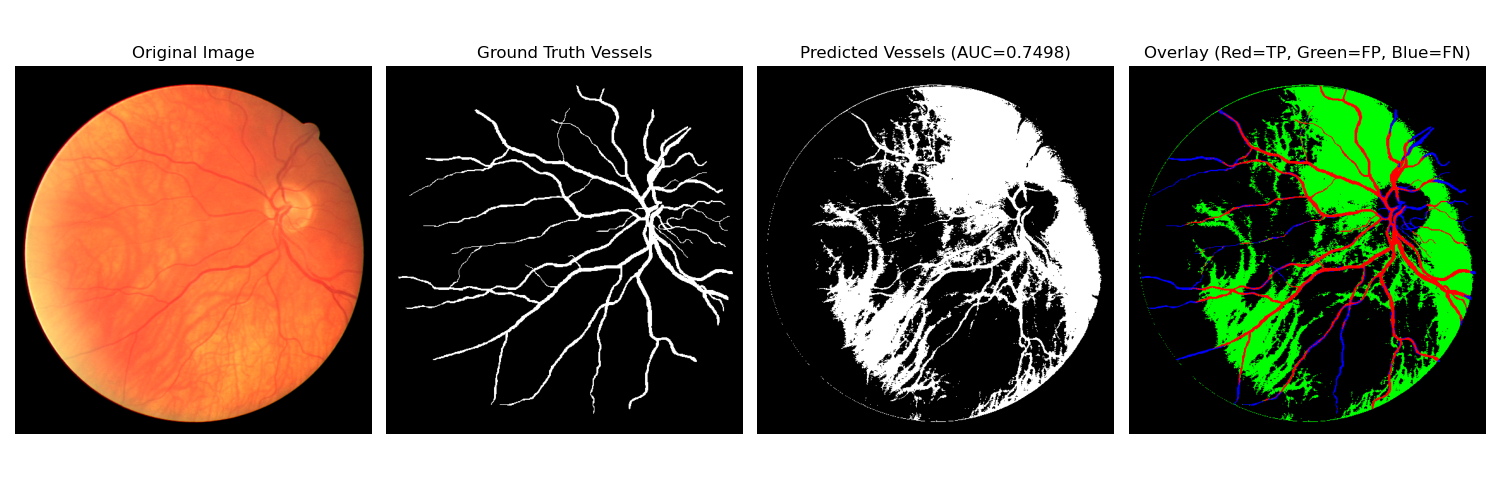
\includegraphics[scale=0.35]{Figures/3 Optmized 1st.png}
    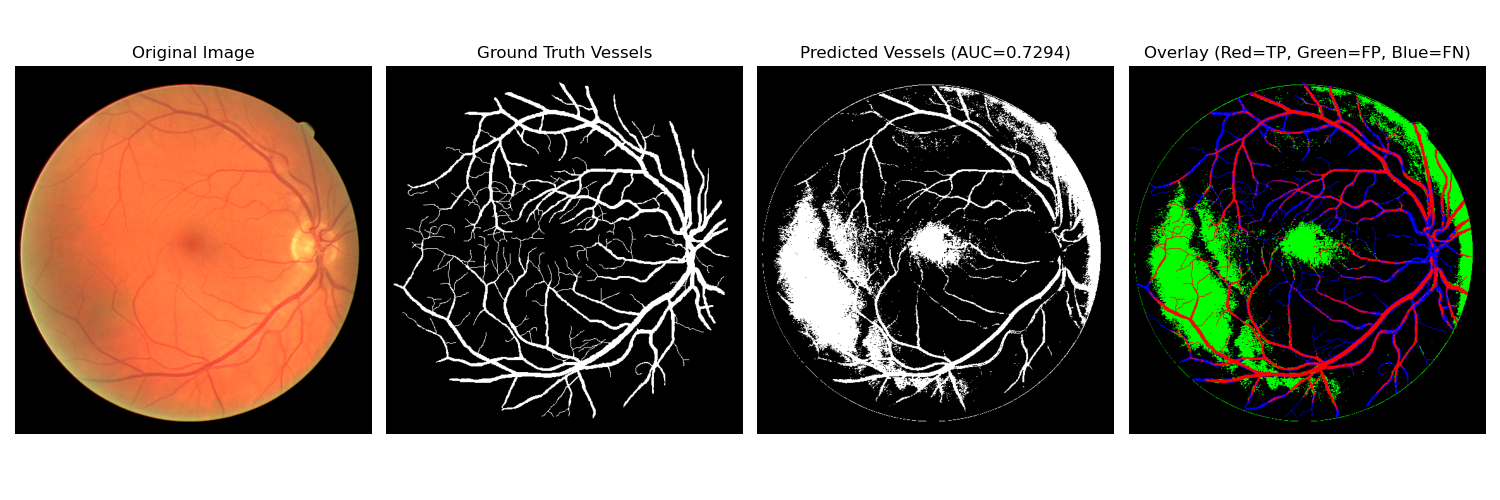
\includegraphics[scale=0.35]{Figures/3 Optmized 2nd.png}
    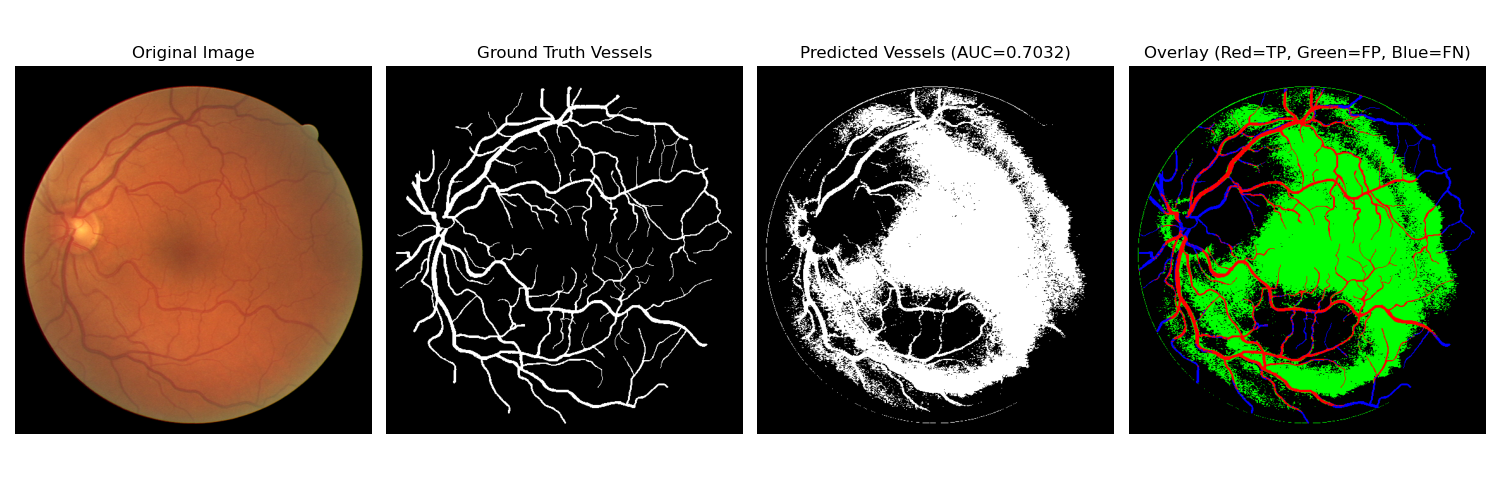
\includegraphics[scale=0.35]{Figures/3 Optmized 3rd.png}
\end{center}


\subsubsection{Use the Optimized K-means Algorithm with the Image Augmentation}
The best three examples are:
\begin{center}
    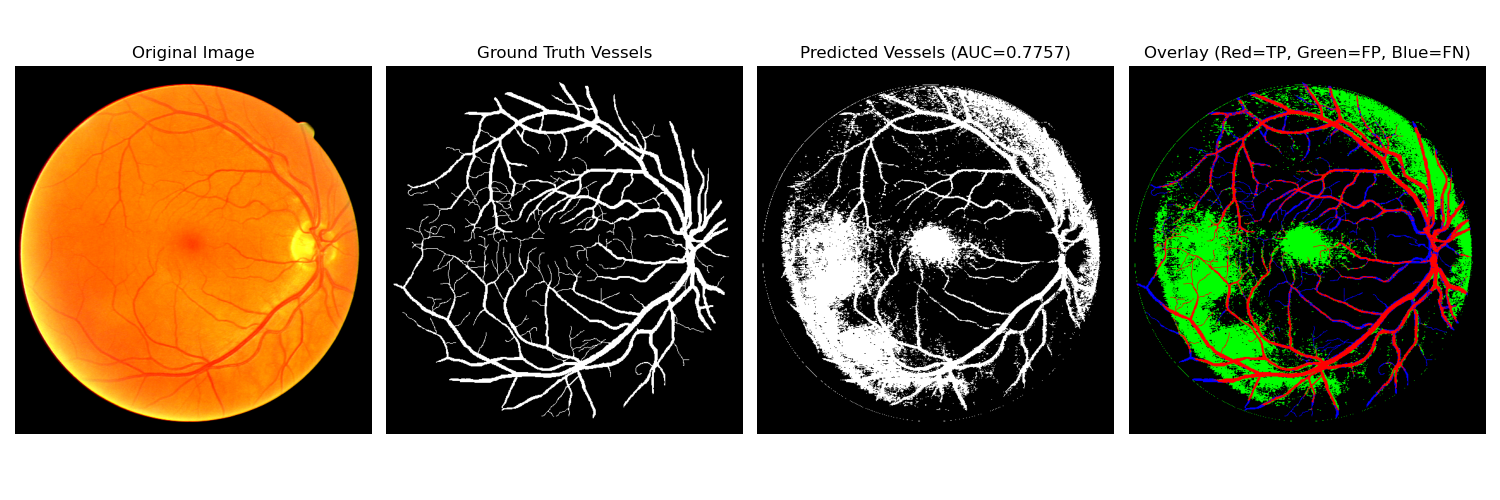
\includegraphics[scale=0.35]{Figures/4 Optmized 1st.png}
    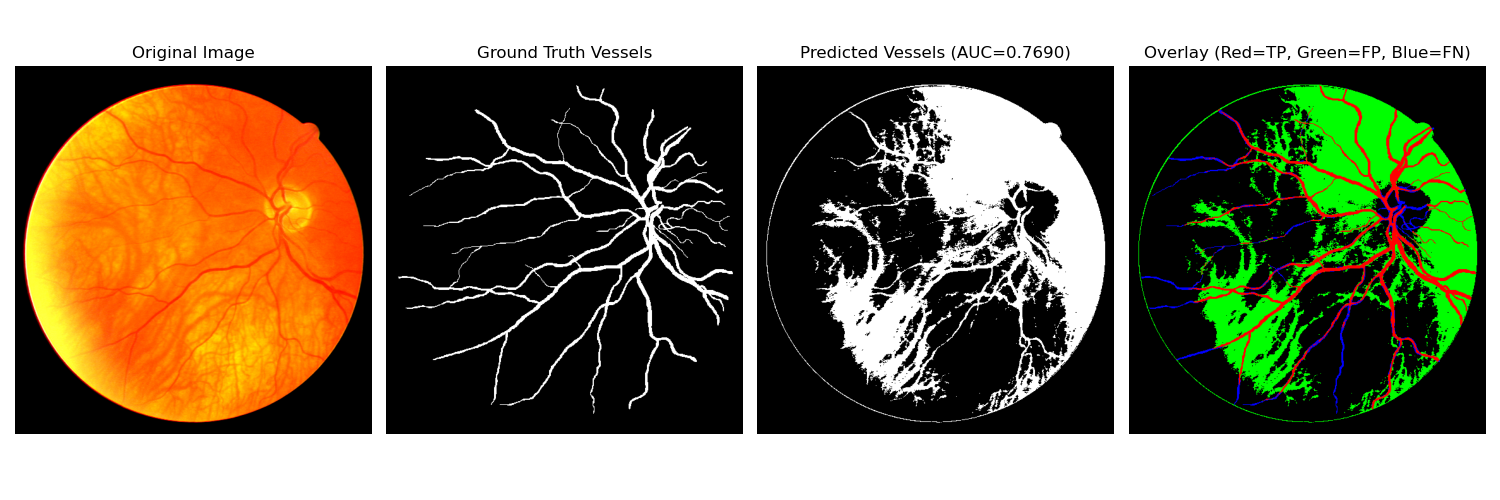
\includegraphics[scale=0.35]{Figures/4 Optmized 2nd.png}
    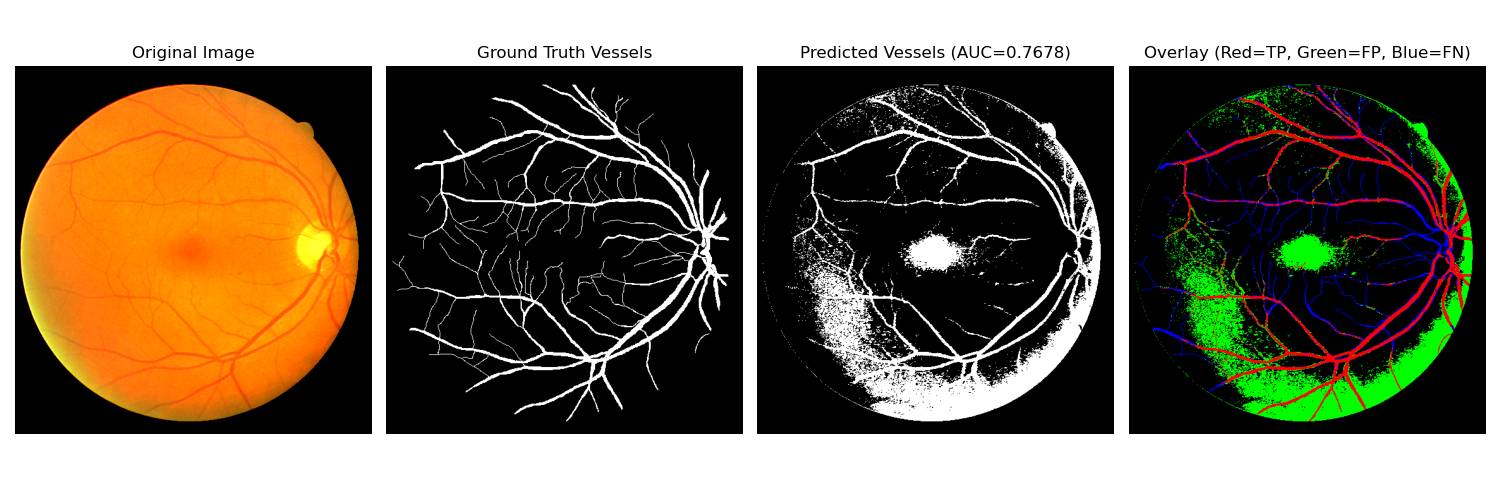
\includegraphics[scale=0.35]{Figures/4 Optmized 3rd.png}
\end{center}


\subsubsection{Performance Comparison}
\begin{table}[H]
    \centering
    \caption{Performance Comparison: Before and After Image Augmentation}
    \begin{tabular}{lcc}
    \hline
    \textbf{Metric} & \textbf{Classic KMeans} & \textbf{Optimized KMeans} \\
    \hline
    Accuracy & $0.8575 \rightarrow \textcolor{red}{0.8758}$ & $0.7266 \rightarrow \textcolor{red}{0.7673}$ \\
    Sensitivity & $0.2366 \rightarrow \textcolor{red}{0.3024}$ & $0.6042 \rightarrow \textcolor{red}{0.6493}$ \\
    Specificity & $0.9165 \rightarrow \textcolor{red}{0.9304}$ & $0.7385 \rightarrow \textcolor{red}{0.7789}$ \\
    F1 & $0.2278 \rightarrow \textcolor{red}{0.3047}$ & $0.2782 \rightarrow \textcolor{red}{0.3292}$ \\
    Auc & $0.5766 \rightarrow \textcolor{red}{0.6164}$ & $0.6714 \rightarrow \textcolor{red}{0.7141}$ \\
    \hline
    \end{tabular}
\end{table}



\subsubsection{Direction-enhanced KMeans Clustering}
The best examples with merging the top 3 and 5 clusters are: 
\begin{center}
    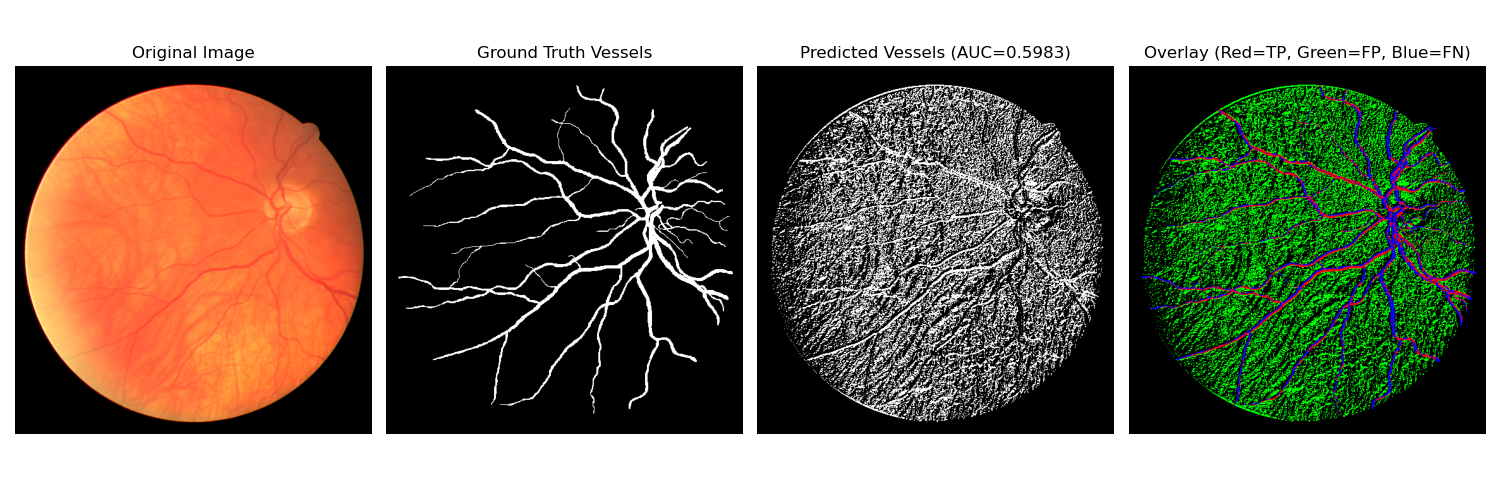
\includegraphics[scale=0.35]{Figures/5 Directed (Merge 3 Clusters).png}
    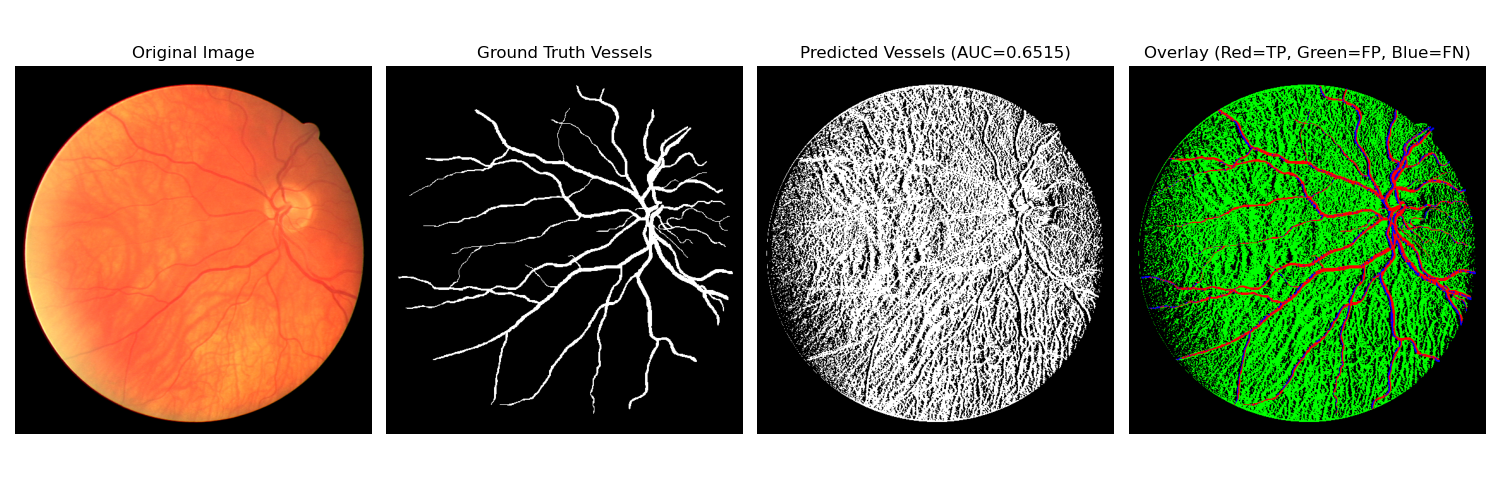
\includegraphics[scale=0.35]{Figures/5 Directed (Merge 5 Clusters).png}
\end{center}
After applying the image augmentation:
\begin{center}
    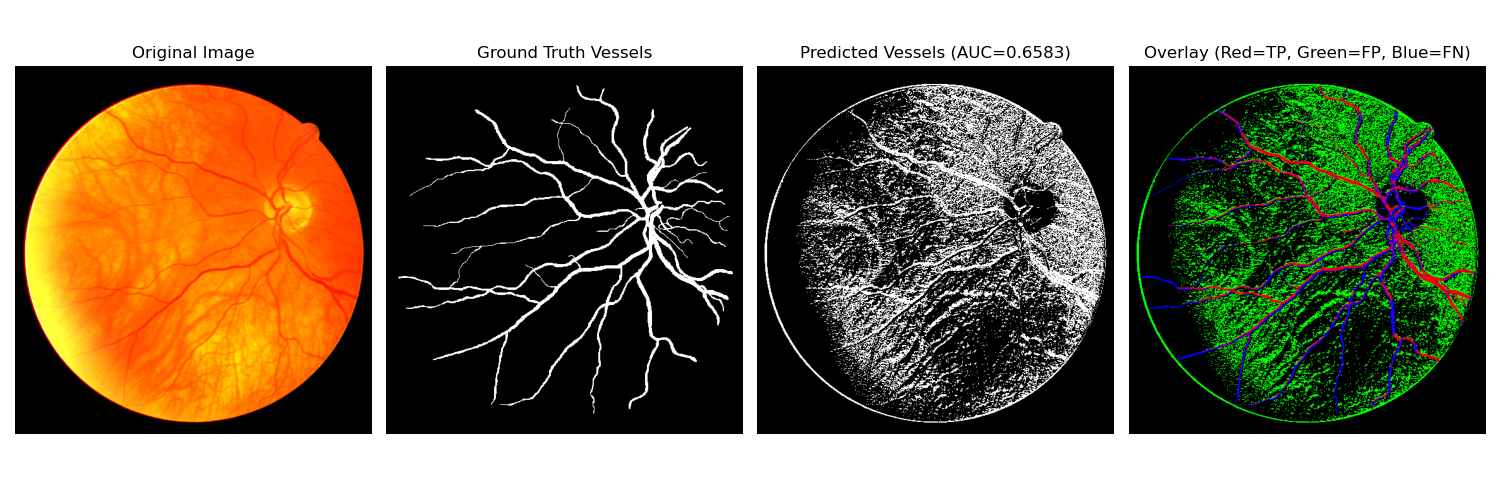
\includegraphics[scale=0.35]{Figures/6 Directed (Merge 3 Clusters).png}
    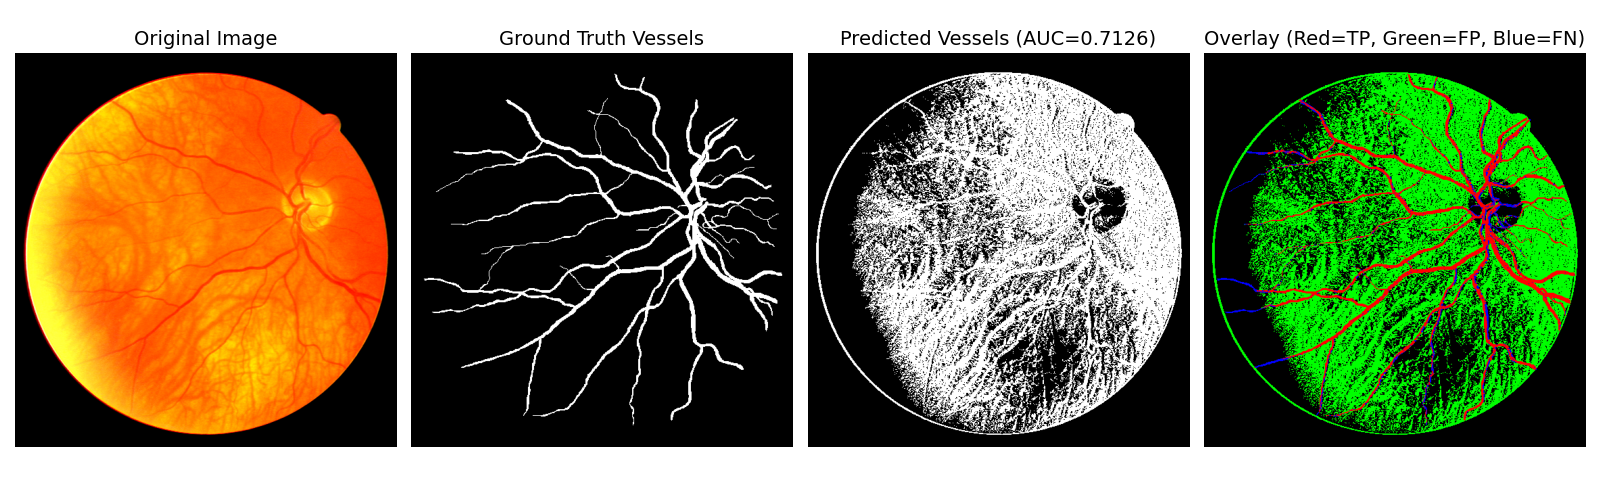
\includegraphics[scale=0.35]{Figures/6 Directed (Merge 5 Clusters).png}
\end{center}








\end{document}
